\section{Banco de Dados Original}
\begin{frame}{Formato dos Dados}
    \begin{itemize}[itemsep = 5em]
        \item Planilhas no formato csv dos anos de 1963 até 2015 com os dados 
            de alunos da UnB
    \end{itemize}
\end{frame}

\begin{frame}{Dados de Interesse}
    \begin{itemize}
        \item Dados de perfil dos alunos 
        \item Ano e semestre de ingresso 
        \item Ano e semestre que saiu 
        \item Forma de ingresso e forma de saída
        \item Matérias que pegou em um dado semestre e suas respectivas menções
    \end{itemize}
\end{frame}

\begin{frame}{Modelagem do BD}
            \begin{figure}[!ht]
                \caption{Modelo entidade relacionamento do BD}
                \centering
                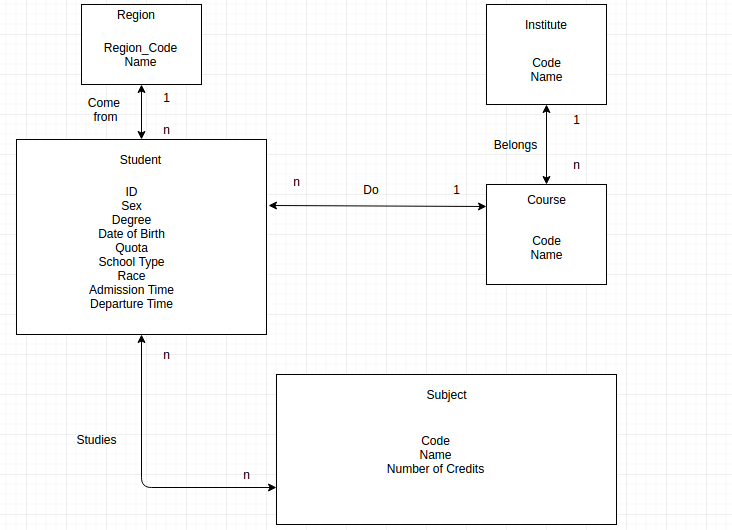
\includegraphics[width = 8cm]{./images/database.png}
            \end{figure}
\end{frame}
